\section{欧拉函数}
\subsection{欧拉函数}
\begin{frame}[fragile]{欧拉函数}{基本概念}
  \textbf{定义}:欧拉函数,即$\varphi(n)$,表示小于等于$n$且和$n$互质的数的个数。特别地,$\varphi(1)=1$。
  $$
  \varphi(n) = \sum\limits_{i=1}^{n} [\gcd(i, n)=1]
  $$
  显然,当$n$是质数时,$\varphi(n)=n-1$。
  \vspace{0.3cm}
  \pause

  \textbf{性质}:
  \begin{itemize}
    \item 欧拉函数是\textbf{积性函数}(证明:\href{https://xdbirdie.github.io/2020/07/07/%E6%AC%A7%E6%8B%89%E5%87%BD%E6%95%B0/}{欧拉函数的积性证明})
    \begin{itemize}
      \item \textbf{积性函数}:若$f(n)$是积性函数,那么当$\gcd(a,b)=1$时,有$f(a\cdot b)=f(a)\cdot f(b)$。
      \item \textbf{完全积性函数}:若$f(n)$是完全积性函数,那么有$f(a\cdot b)=f(a)\cdot f(b)$
    \end{itemize}
    \pause
    \item $n = \sum_{d|n}\varphi(d)$。由\textbf{莫比乌斯反演}可得。
    \pause
    \item 若$n=p^k$,其中$p$是质数,那么$\varphi(n)=p^k - p^{k-1}$。
    \item 由唯一分解定理,设 $n = \prod_{i=1}^{n}p_i^{k_i}$,其中 $p_i$ 是质数,有 $\varphi(n) = n \cdot \prod\limits_{i = 1}^s{\dfrac{p_i - 1}{p_i}}$。
  \end{itemize}
\end{frame}

\begin{frame}[fragile]{欧拉函数}{求解}
  \begin{itemize}
    \item \textbf{求解单个欧拉函数值}:直接质因数分解就好了
    \begin{lstlisting}
    int phi(int n) {
      int ans = n;
      for (int i = 2; i * i <= n; i++)
        if (n % i == 0) {
          ans = ans / i * (i - 1);
          while (n % i == 0) n /= i;
        }
      if (n > 1) ans = ans / n * (n - 1);
      return ans;
    }
    \end{lstlisting}
  \end{itemize}
\end{frame}

\begin{frame}[fragile]{欧拉函数}{求解}
  \begin{itemize}
    \item \textbf{求解$1\sim n$的欧拉函数值}:线性筛
    \begin{lstlisting}
void init() {
  int cnt = 0;
  phi[1] = 1;
  for (int i = 2; i < MAXN; i++) {
    if (!inp[i]) {
      prime[++cnt] = i;
      phi[i] = i - 1;
    }

    for (int j = 1; j <= cnt && i * prime[j] < MAXN; j++) {
      inp[i * prime[j]] = true;
      if (i % prime[j] == 0) {
        phi[i * prime[j]] = phi[i] * prime[j];
        break;
      }
      else 
        phi[i * prime[j]] = phi[i] * (prime[j] - 1);      
    }
  }
}
    \end{lstlisting}
  \end{itemize}
\end{frame}

\begin{frame}[fragile]{欧拉函数}{例题}
  \textbf{题目链接}:\href{https://www.luogu.com.cn/problem/P2158}{P2158 [SDOI2008]仪仗队 - 洛谷}
  \begin{block}{题目描述}
    \begin{figure}
      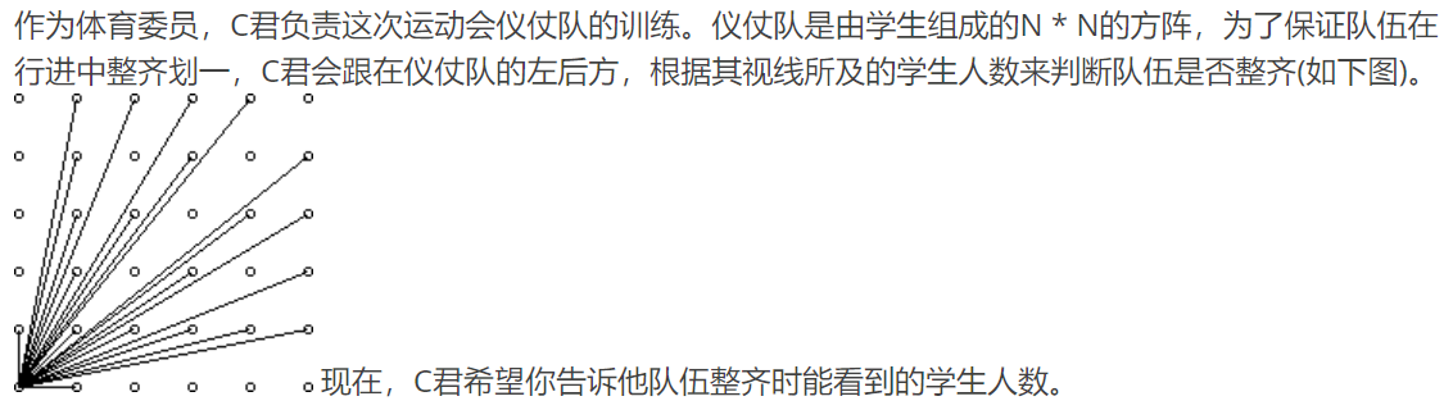
\includegraphics[width=0.7\textwidth]{images/img1.png}
    \end{figure}
  \end{block}

  \pause 
  \begin{exampleblock}{题解}
    \begin{itemize}
      \item 什么时候一个人会被另一个人挡住?
      \pause 
      \item 假设俩人坐标为$(x_1,y_1)$,$(x_2,y_2)$,$x_1\leq x_2$
      \item 显然当且仅当$\frac{y_1}{x_1}=\frac{y_2}{x_2}$时$2$会被$1$挡住
      \pause
      \item 只考虑$y<x$的部分,可得第$i$列只有$\varphi(i)$个人没被挡住,即可被看见
      \pause 
      \item 所以$ans =2*(\sum\limits_{i=1}^n\varphi(i))+1$
    \end{itemize}
  \end{exampleblock}
\end{frame}

\subsection{费马小定理}
\begin{frame}[fragile]{费马小定理}
  \begin{theorem}[费马小定理]
    若 $p$ 为素数,$\gcd(a, p) = 1$,则 $a^{p - 1} \equiv 1 \pmod{p}$。\\
    另一个形式:对于任意整数 $a$,有 $a^p \equiv a \pmod{p}$。
  \end{theorem}
  \pause 
  \vspace{0.5cm}

  费马小定理常用于结合\textbf{快速幂}求解\textbf{乘法逆元}:
  $$
  a^{p-2}\cdot a \equiv 1 \pmod{p}, (\gcd(a,p)=1)
  $$

  \pause
  \vspace{0.5cm}
  \textbf{证明}:\sout{我有一个对这个命题的十分美妙的证明,这里空白太小,我写不下了。}
\end{frame}

\begin{frame}[fragile]{费马小定理}{证明}
  \begin{proof}
    设一个质数为 $p$,且$\gcd(a,p)=1$。\\
    构造一个序列:$A=\{1,2,3\dots,p-1\}$,这个序列有着这样一个性质:
    $$
    \prod_{i=1}^{n}\space A_i\equiv\prod_{i=1}^{n} (A_i\times a) \pmod p
    $$
    
    \pause 
    思路:反证法可证得$\forall i\neq j,A_i a\not\equiv A_ja \pmod{p}$
    \\ 那么$\{A_ia\}$将取到$1\sim p-1$内的所有值。
    
    \pause 
    $$
    \begin{aligned}
      & \prod_{i=1}^{n}(A_i\times a) &\equiv\prod_{i=1}^{n} A_i &\pmod{p}\\
      \Rightarrow & a^{p-1}\prod_{i=1}^{n} A_i &\equiv\prod_{i=1}^{n} A_i &\pmod{p}\\
      \Rightarrow & a^{p-1} &\equiv 1 &\pmod{p}
    \end{aligned}
    $$
  \end{proof}
\end{frame}

\subsection{欧拉定理}
\begin{frame}[fragile]{欧拉定理}
  \begin{theorem}[欧拉定理]
    若 $\gcd(a, m) = 1$,则 $a^{\varphi(m)} \equiv 1 \pmod{m}$。
  \end{theorem}
  则当$m$为质数时,$\varphi(m)=m-1$,则可得$a^{m-1}\equiv 1 \pmod{m}$,即得到了费马小定理。
  
  \pause 
  \vspace{1.0cm}
  \textbf{证明}:\href{https://xdbirdie.github.io/2020/07/10/%E6%AC%A7%E6%8B%89%E5%AE%9A%E7%90%86%E4%B8%8E%E8%B4%B9%E9%A9%AC%E5%B0%8F%E5%AE%9A%E7%90%86/}{欧拉定理与费马小定理及证明}
\end{frame}

\begin{frame}[fragile]{拓展欧拉定理}
  欧拉定理只能在$\gcd(a,p)=1$时使用,限制很大。
  \pause
  \begin{theorem}[拓展欧拉定理]
    \begin{equation*}
      a^{b} \equiv\left\{\begin{array}{ll}
      a^{b \bmod \varphi(p)}, & \operatorname{gcd}(a, p)=1 \\
      a^{b}, & \operatorname{gcd}(a, p) \neq 1, b<\varphi(p) \quad(\bmod p) \\
      a^{b \bmod \varphi(p)+\varphi(p)}, & \operatorname{gcd}(a, p) \neq 1, b \geq \varphi(p)
      \end{array}\right.
    \end{equation*}
  \end{theorem}

  \pause 
  \vspace{0.3cm}
  完美满足所有情况,非常好用。\sout{(虽然我没怎么用过)}
  
  \pause
  \vspace{0.3cm}
  \textbf{证明}:\sout{太长了我写不下}\hspace{0.3cm} \sout{我不会}

  \pause 
  \vspace{0.3cm}
  常用于\textbf{欧拉降幂}。

\end{frame}

\begin{frame}[fragile]{拓展欧拉定理}{例题}
  \textbf{题目链接}:\href{https://acm.xidian.edu.cn/problem.php?id=1066}{P1066 A\^B\%P - XDOJ}
  \begin{block}{题目描述}
    求解:
    $$
    (\dots ((A^{B_0})^{B_1})\dots)^{B_{n-1}}\bmod{P}
    $$
    其中,$B_i=B_{i-1}^2-1(i>0)$,$P=1e9+7$。\\
    数据范围:$0<A<2^{31},0\le n\le 1e5,1<B_0<2^{31}$
  \end{block}
  \pause
  \begin{exampleblock}{题解}
    \begin{itemize}
      \item 即求$A^{\sum\limits_{i=0}^{n-1}B_i}\bmod{p}$,但是$B_i$是指数级增加,无法直接求出
      \pause 
      \item 显然\textbf{欧拉降幂},考虑适用条件
      \item $P=1e9+7$是质数,所以要么$\gcd(A,P)=1$,要么$P|A$
      \pause 
      \item 显然二者条件下,$A^{x}\equiv A^{x\bmod \varphi(P)} \pmod{P}$均成立
      \item 所以先求出$\sum\limits_{i=0}^{n-1}B_i\bmod{\varphi(P)}\;\;\;\;(\varphi(P)=P-1)$即可。
    \end{itemize}
  \end{exampleblock}
\end{frame}